\chapter{Appendix}
    \section{AndroidThings}
    \begin{lstlisting}[
        caption={Android studio gradle file example},
        label={code:gradleExample},
        language=java
        ]
        apply plugin: 'com.android.application'
        apply plugin: 'com.neenbedankt.android-apt'
        android {
            compileSdkVersion 26
            buildToolsVersion "26.0.2"
            defaultConfig {
                applicationId "navigation.egd.haw.egd_navigation_cj2"
                minSdkVersion 24
                targetSdkVersion 26
                versionCode 1
                versionName "1.0"
                testInstrumentationRunner "android.support.test.
                runner.AndroidJUnitRunner"
            }
            buildTypes {
                release {
                    minifyEnabled false
                    proguardFiles getDefaultProguardFile('proguard-android.txt'),
                     'proguard-rules.pro'
                }
            }
        }
        
        dependencies {
            compile fileTree(dir: 'libs', include: ['*.jar'])
            androidTestCompile('com.android.support.test.espresso:
            espresso-core:2.2.2', 
            {
                exclude group: 'com.android.support', module: 
                'support-annotations'
            })
            compile 'com.android.support:appcompat-v7:26.+'
            compile 'com.android.support.constraint:constraint-layout:1.0.2'
            testCompile 'junit:junit:4.12'
        
            //Android Things
            //here should be the version of android things you want to use
            provided 'com.google.android.things:androidthings:0.5.1-devpreview'
        
            //network
            compile 'com.squareup.retrofit2:retrofit:2.1.0'
            compile 'com.squareup.retrofit2:converter-gson:2.1.0'
        
            // Dependency Injection
            compile "com.google.dagger:dagger:2.6"
            provided 'javax.annotation:jsr250-api:1.0'
            apt "com.google.dagger:dagger-compiler:2.6"
        
            //Xml Reader
            compile('org.simpleframework:simple-xml:2.7.+'){
                exclude module: 'stax'
                exclude module: 'stax-api'
                exclude module: 'xpp3'
            }
        }
         
    \end{lstlisting} 
    \section{Dagger}
        \label{appendix:dagger}
        Dagger is dependency injection framework. It is based on the 
        Java Specification Request (JSR) 330. 
        It uses code generation and is based 
        on annotations. The generated code is very relatively easy to read 
        and debug. It is the most popular dependency injection framework
        for android also used for java projects only.


    \begin{figure}[htbp!]
        \centering 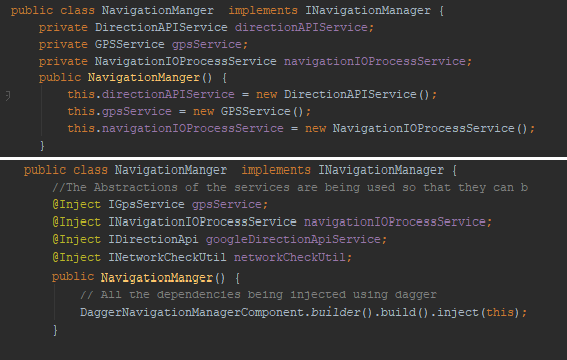
\includegraphics{grafiken/di_compare.png}
        \caption{Comparision of code with(bottom) and without Dependency injection(top)}
        \label{fig:DIComparision}
    \end{figure}

    